\documentclass[12pt]{article}
\usepackage{../../ficha}

\begin{document}

\ficha{Limites de Funções e Continuidade}[Indeterminações, Limites Notáveis, Assíntotas e Teorema de Bolzano]

\instrucoes{Resolve os exercícios, levantando as indeterminações. Limites notáveis: $\displaystyle\lim_{x \to 0}\dfrac{\sin x}{x} = 1$, $\;\displaystyle\lim_{x \to 0}\dfrac{e^x - 1}{x} = 1$, $\;\displaystyle\lim_{x \to +\infty}\dfrac{e^x}{x^p} = +\infty$ e $\;\displaystyle\lim_{x \to +\infty}\dfrac{\ln x}{x} = 0$.}

\secao{Limites a Partir de Gráficos}{Observa o gráfico de $f$ e indica os limites.}

\begin{center}
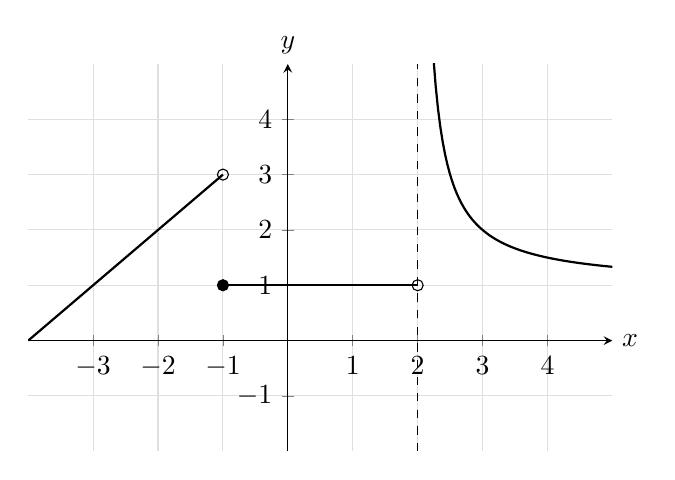
\begin{tikzpicture}
\begin{axis}[axis lines=middle, xmin=-4, xmax=5, ymin=-2, ymax=5, xtick={-3,...,4}, ytick={-1,...,4}, grid=both, grid style={gray!25}, width=9cm, height=6.5cm, xlabel=$x$, ylabel=$y$, every axis x label/.style={at={(ticklabel* cs:1)},anchor=west}, every axis y label/.style={at={(ticklabel* cs:1)},anchor=south}]
  \addplot[thick, domain=-4:-1] {x + 4};
  \addplot[thick, domain=-1:2] {1};
  \addplot[thick, domain=2.17:5, samples=80] {1/(x-2) + 1};
  \addplot[only marks, mark=*, mark size=2pt] coordinates {(-1,1)};
  \addplot[only marks, mark=o, mark size=2pt, fill=white] coordinates {(-1,3) (2,1)};
  \draw[dashed] (axis cs:2,-2) -- (axis cs:2,5);
\end{axis}
\end{tikzpicture}
\end{center}

\begin{exercicios}
  \item $\displaystyle\lim_{x \to -1^-} f(x)$ \; e \; $\displaystyle\lim_{x \to -1^+} f(x)$. Existe $\displaystyle\lim_{x \to -1} f(x)$?
  \item $f(-1)$. A função é contínua em $x = -1$?
  \item $\displaystyle\lim_{x \to 2^-} f(x)$ \; e \; $\displaystyle\lim_{x \to 2^+} f(x)$
  \item $\displaystyle\lim_{x \to +\infty} f(x)$
  \item Indica as equações das assíntotas do gráfico de $f$ visíveis na figura.
\end{exercicios}

\secao{Indeterminações $\dfrac{0}{0}$}{Calcula.}
\begin{exercicios}
  \item $\displaystyle\lim_{x \to 2} \dfrac{x^2 - 4}{x - 2}$
  \item $\displaystyle\lim_{x \to 3} \dfrac{x^2 - 5x + 6}{x - 3}$
  \item $\displaystyle\lim_{x \to -1} \dfrac{x^2 - 1}{x^2 + 3x + 2}$
  \item $\displaystyle\lim_{x \to 1} \dfrac{x^3 - 1}{x - 1}$
  \item $\displaystyle\lim_{x \to 4} \dfrac{\sqrt{x} - 2}{x - 4}$
  \item $\displaystyle\lim_{x \to 0} \dfrac{\sqrt{x + 9} - 3}{x}$
\end{exercicios}

\secao{Limites no Infinito}{Calcula.}
\begin{exercicios}
  \item $\displaystyle\lim_{x \to +\infty} \dfrac{3x^2 - x}{x^2 + 4}$
  \item $\displaystyle\lim_{x \to -\infty} \dfrac{2x + 1}{x^2 - 3}$
  \item $\displaystyle\lim_{x \to +\infty} \dfrac{x^3 + 1}{5x - 2}$
  \item $\displaystyle\lim_{x \to +\infty} \left(\sqrt{x^2 + x} - x\right)$
  \item $\displaystyle\lim_{x \to -\infty} \dfrac{\sqrt{x^2 + 1}}{x}$
  \item $\displaystyle\lim_{x \to 2^-} \dfrac{1}{x - 2}$ \; e \; $\displaystyle\lim_{x \to 2^+} \dfrac{1}{x - 2}$
\end{exercicios}

\secao{Limites Notáveis}{Calcula.}
\begin{exercicios}
  \item $\displaystyle\lim_{x \to 0} \dfrac{\sin(3x)}{x}$
  \item $\displaystyle\lim_{x \to 0} \dfrac{\sin(5x)}{\sin(2x)}$
  \item $\displaystyle\lim_{x \to 0} \dfrac{\tan x}{x}$
  \item $\displaystyle\lim_{x \to 0} \dfrac{1 - \cos x}{x^2}$
  \item $\displaystyle\lim_{x \to 0} \dfrac{e^{2x} - 1}{x}$
  \item $\displaystyle\lim_{x \to 0} \dfrac{\ln(1 + x)}{x}$
  \item $\displaystyle\lim_{x \to +\infty} \dfrac{e^x}{x^3}$
  \item $\displaystyle\lim_{x \to +\infty} \dfrac{\ln x}{\sqrt{x}}$
  \item $\displaystyle\lim_{x \to +\infty} x\,e^{-x}$
  \item $\displaystyle\lim_{x \to 0^+} x \ln x$
\end{exercicios}

\secao{Continuidade e Assíntotas}{Resolve.}
\begin{exercicios}
  \item Estuda a continuidade de $f(x) = \begin{cases} \dfrac{x^2 - 9}{x - 3} & \text{se } x \neq 3 \\ 6 & \text{se } x = 3 \end{cases}$
  \item Determina $k$ de modo que $f(x) = \begin{cases} \dfrac{\sin(2x)}{x} & \text{se } x < 0 \\ x + k & \text{se } x \ge 0 \end{cases}$ seja contínua em $x = 0$.
  \item Determina as assíntotas verticais e horizontais de $f(x) = \dfrac{2x + 1}{x - 3}$.
  \item Determina as assíntotas do gráfico de $f(x) = \dfrac{x^2 + 1}{x}$ (incluindo a oblíqua).
  \item Determina a assíntota oblíqua de $f(x) = \dfrac{2x^2 - 3x + 1}{x + 1}$.
  \item Determina as assíntotas horizontais de $f(x) = \dfrac{e^x}{e^x + 1}$.
\end{exercicios}

\secao{Teorema de Bolzano-Cauchy}{Resolve.}
\begin{exercicios}
  \item Mostra que a equação $x^3 + x - 1 = 0$ tem pelo menos uma solução em $]0, 1[$.
  \item Mostra que $f(x) = x^3 - 3x + 1$ tem pelo menos três zeros. (Sugestão: calcula $f(-2)$, $f(0)$, $f(1)$ e $f(2)$.)
  \item Mostra que a equação $\cos x = x$ tem pelo menos uma solução em $\left]0, \dfrac{\pi}{2}\right[$.
  \item Usando o método da bisseção, determina um valor aproximado às décimas da solução de $x^3 + x - 1 = 0$.
  \item Mostra que $e^x = 3 - x$ tem uma solução em $]0, 1[$.
\end{exercicios}

\secao{Desafios}{Resolve os problemas.}
\begin{exercicios}
  \item Determina $a$ e $b$ de modo que $\displaystyle\lim_{x \to 1} \dfrac{x^2 + ax + b}{x - 1} = 5$.
  \item Calcula $\displaystyle\lim_{x \to +\infty} \left(1 + \dfrac{2}{x}\right)^{x}$.
  \item Calcula $\displaystyle\lim_{x \to 0} \dfrac{x \sin x}{1 - \cos x}$.
  \item Pelo teorema de Weierstrass, mostra que $f(x) = x^2 - 2x$ tem máximo e mínimo em $[0, 3]$ e determina-os.
\end{exercicios}

\end{document}
